\begin{surferPage}[Sept-Sim]{O septic\u{a} simetric\u{a}}

     Aceast\u{a} suprafa\c{t}\u{a} care arat\u{a} ca o stea are grad $7$.
     Are $84$ de singularit\u{a}\c{t}i, numarul maxim de singularit\u{a}\c{t}i 
     reale cunoscute pentru septice p\^{a}n\u{a} de cur\^{a}nd; doar 
     \^{i}n 2004, Oliver Labs a \^{i}mbun\u{a}t\u{a}\c{t}it acest record la $99$.
     
  Cele trei perne care pot fi v\u{a}zute \^{i}n imaginea interactiv\u{a} 
    se datoreaz\u{a} folosirii polinoamelor Chebychev, similar cu octica lui Chmutov.
    De fapt, aceast\u{a} suprafa\c{t}\u{a} este o alt\u{a} variant\u{a} a suprafe\c{t}ei lui Chmutov. Aici,
    curba plan\u{a} $T_d(x)+T_d(y)$ este inlocuit\u{a} de heptagonul regulat $S_7(x,y)$: 
   \[S_7(x,y) + \lambda \cdot T_d(z) = 0,\]
    pentru o valoare convenabil\u{a} $\lambda\in\RR$. 
      \vspace*{-0.3em}
    \begin{center}
      \begin{tabular}{c@{\qquad}c}
        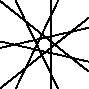
\includegraphics[height=1.5cm]{./../../common/images/labsseptic1.pdf}
        &
        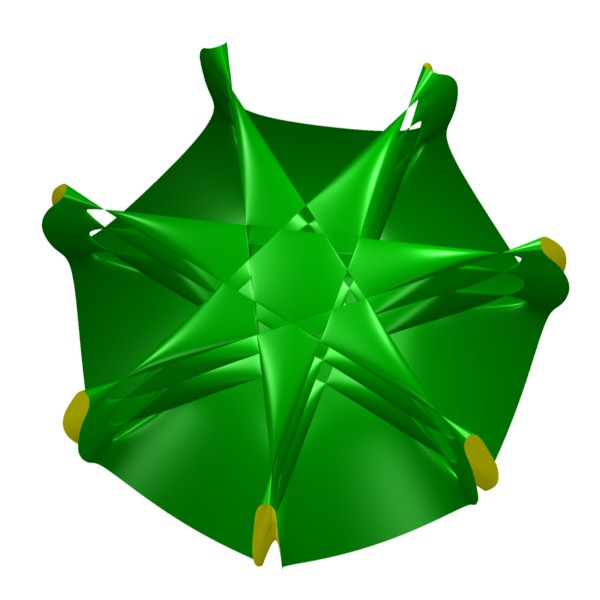
\includegraphics[height=1.5cm]{./../../common/images/septic_7eck_von_oben}
      \end{tabular}
    \end{center}
    \vspace*{-0.3em}   
   Aceast\u{a} variant\u{a} a construc\c{t}iei lui Chmutov se datoreaz\u{a} lui Duco van Straten.

\end{surferPage}
